% Journal-ready LaTeX manuscript generated from the thesis results.
% Compile from repository root:
%   cd paper && pdflatex main_paper.tex && pdflatex main_paper.tex

\documentclass[11pt]{article}
\usepackage[a4paper,margin=1in]{geometry}
\usepackage{times}
\usepackage{microtype}
\usepackage{authblk}
\usepackage{graphicx}
\usepackage{booktabs}
\usepackage{tabularx}
\usepackage{array}
\usepackage{amsmath,amssymb}
\usepackage{caption}
\usepackage{float}
\usepackage[hidelinks]{hyperref}
\usepackage{enumitem}

\graphicspath{{../results/figures/}{../results/}{./figures/}{./}}
\newcommand{\modelname}{ETHOS}
\newcommand{\mimic}{MIMIC-IV v3.1}
\newcommand{\auroc}{AUROC}
\newcommand{\auprc}{AUPRC}
\newcommand{\ci}[2]{[#1, #2]}

\title{\textbf{Symptom-Token Few-Shot Learning for Privacy-Preserving Treatment Feasibility Prediction in Intensive Care: A Reproducible MIMIC-IV Study}}
\author[1]{Mohammad Sharafi}
\author[1]{Gholamreza Aminian}
\affil[1]{Department of Computer Engineering, Islamic Azad University, Tehran North Branch, Tehran, Iran}
\date{}

\begin{document}
\maketitle

\begin{abstract}
\textbf{Background:} Clinical machine-learning models often depend on large centralized datasets, yet intensive-care data are sensitive, heterogeneous, and institutionally siloed. This study evaluates treatment-feasibility prediction in the intensive care unit (ICU), operationalized as predicting a measurable discharge-related clinical outcome from early ICU signals, not as recommending treatment or replacing clinician judgment.

\textbf{Methods:} We constructed a reproducible benchmark using 2,000 adult ICU patients from \mimic{} across five disease nodes: sepsis, cardiovascular, respiratory, renal, and diabetes-related conditions. Early laboratory values and vital signs were represented through a tabular pathway with 25 engineered clinical features and a neural pathway using compact Symptom Tokens encoded by \modelname{}, a transformer-based health-outcome encoder. We evaluated classical tabular models, episodic few-shot learning, hybrid \modelname{}-tabular representations, stacked meta-learning, ablation settings, cross-disease generalization, calibration, interpretability, and a simulated federated-learning setting using FedAvg.

\textbf{Results:} The strongest tabular pipeline achieved test \auroc{} 0.748, F1 0.674, accuracy 0.700, and MCC 0.348. The best few-shot submodel alone reached \auroc{} 0.670, showing that raw few-shot learning did not directly replace strong tabular baselines. A stacked hybrid model combining few-shot probabilities, Random Forest probabilities, and learned representations achieved \auroc{} 0.746 with a 95\% bootstrap confidence interval of \ci{0.699}{0.797}, reducing the point-estimate gap to the tabular ceiling to 0.002 \auroc{}. In a separate fixed-protocol comparison, the proposed few-shot model reached 0.611 \auroc{} compared with 0.762 for Random Forest. Simulated federated training introduced a small utility cost of approximately 0.005 \auroc{} relative to centralized training.

\textbf{Conclusions:} Few-shot learning alone is insufficient for robust treatment-feasibility prediction on limited structured ICU data. However, symptom-token representations, transformer embeddings, and stacked fusion can approach the performance of strong classical baselines while enabling a privacy-preserving federated-learning pathway.
\end{abstract}

\noindent\textbf{Keywords:} few-shot learning; clinical machine learning; MIMIC-IV; intensive care; federated learning; symptom tokens; transformer; treatment feasibility; biomedical informatics.

\section{Introduction}
Clinical decision-making in intensive care is urgent, high-stakes, and data-rich. During the first 24--48 hours of ICU admission, clinicians integrate laboratory trends, vital signs, organ-function markers, and discharge-readiness signals. Machine-learning models may support this process by ranking patients according to probable favorable discharge-related trajectories, but they must remain decision-support tools rather than autonomous treatment systems.

A major barrier in clinical machine learning is data access. High-performing models often benefit from centralized datasets, whereas real-world health data are fragmented across institutions and protected by strict privacy constraints. Federated learning addresses this problem by allowing distributed model training without directly exchanging raw patient data. Few-shot learning is also attractive because it aims to adapt from limited support examples. Yet methods that work well in vision or language do not automatically transfer to structured ICU data, where variables are sparse, heterogeneous, and clinically engineered.

This paper asks whether symptom-token few-shot learning can support treatment-feasibility prediction in ICU data. Our central claim is deliberately conservative: few-shot learning is not a standalone replacement for classical tabular models, but it can become valuable as a representation-learning module inside a stacked, privacy-aware clinical prediction system.

\section{Related Work}
Large de-identified EHR datasets such as MIMIC-IV enable reproducible ICU prediction research. Classical models such as Logistic Regression, Random Forest, and gradient boosting remain strong baselines for structured clinical tasks because they handle nonlinear feature interactions and threshold-like clinical effects. Transformer models have also been adapted to EHR sequences, while few-shot learning methods such as Prototypical Networks, Matching Networks, Relation Networks, and MAML-style methods attempt to generalize from small support sets. Federated learning, especially FedAvg, enables privacy-preserving distributed training but introduces challenges including non-IID data, site-specific missingness, calibration drift, and governance.

\section{Methods}
\subsection{Cohort and task}
We used a retrospective cohort of 2,000 adult ICU patients from \mimic{}. Inclusion criteria were first ICU stay only, ICU length of stay of at least four hours, age at least 18 years, and availability of a primary ICD-10 diagnosis sufficient for disease-node assignment. Patients were stratified into five disease nodes: sepsis, cardiovascular, respiratory, renal, and diabetes-related conditions. The split was 64\% training, 16\% validation, and 20\% held-out test.

Treatment feasibility was operationalized as a binary discharge-related endpoint derived from early ICU signals. This label is a research proxy for decision support and should not be interpreted as treatment recommendation, discharge automation, or replacement of clinical judgment.

\subsection{Representations}
Early ICU signals from the first 24 hours were encoded in two pathways. The tabular pathway used 25 dimensions: 22 base laboratory/vital-sign variables and 3 engineered clinical features. The neural pathway converted abnormality patterns into Symptom Tokens and passed them through \modelname{}, a transformer encoder producing 128-dimensional patient embeddings.

\subsection{Models}
Classical baselines included Logistic Regression, Random Forest, XGBoost, LightGBM, and CatBoost. Few-shot experiments used binary episodic classification with support and query sets. Hybrid models concatenated the 128-dimensional \modelname{} embedding with the 25-dimensional tabular vector, yielding a 153-dimensional representation. The stacked model combined few-shot probabilities, Random Forest probabilities, and embedding features using a meta-learner.

\subsection{Federated learning}
Federated learning was simulated by partitioning data across disease nodes. Each node trained locally and the server aggregated parameters by FedAvg:
\begin{equation}
\theta_{t+1}=\sum_{k=1}^{K}\frac{n_k}{n}\theta_t^{(k)},
\end{equation}
where $\theta_t^{(k)}$ denotes the local model from node $k$, $n_k$ is local sample size, and $n$ is total sample size.

\subsection{Evaluation}
The primary metric was held-out test \auroc{}. Secondary metrics included \auprc{}, F1, precision, recall, accuracy, MCC, calibration error, per-disease metrics, and bootstrap confidence intervals where available. We report tabular SOTA, Exp1, stacked few-shot, K-shot sensitivity, and federated experiments separately because they answer different questions.

\section{Results}
\subsection{Tabular ceiling}
The strongest tabular result came from a multi-phase SOTA pipeline using classical tuning, ensembling, light Gaussian augmentation, and threshold tuning.

\begin{table}[H]
\centering
\caption{Tabular SOTA pipeline: best held-out test configuration.}
\small
\begin{tabular}{lcccc}
\toprule
Configuration & AUROC & F1 & Accuracy & MCC \\
\midrule
\texttt{aug\_gaussian\_n300\_std0.03} & \textbf{0.748} & \textbf{0.674} & \textbf{0.700} & \textbf{0.348} \\
\bottomrule
\end{tabular}
\label{tab:tabular-sota}
\end{table}

\begin{figure}[H]
\centering
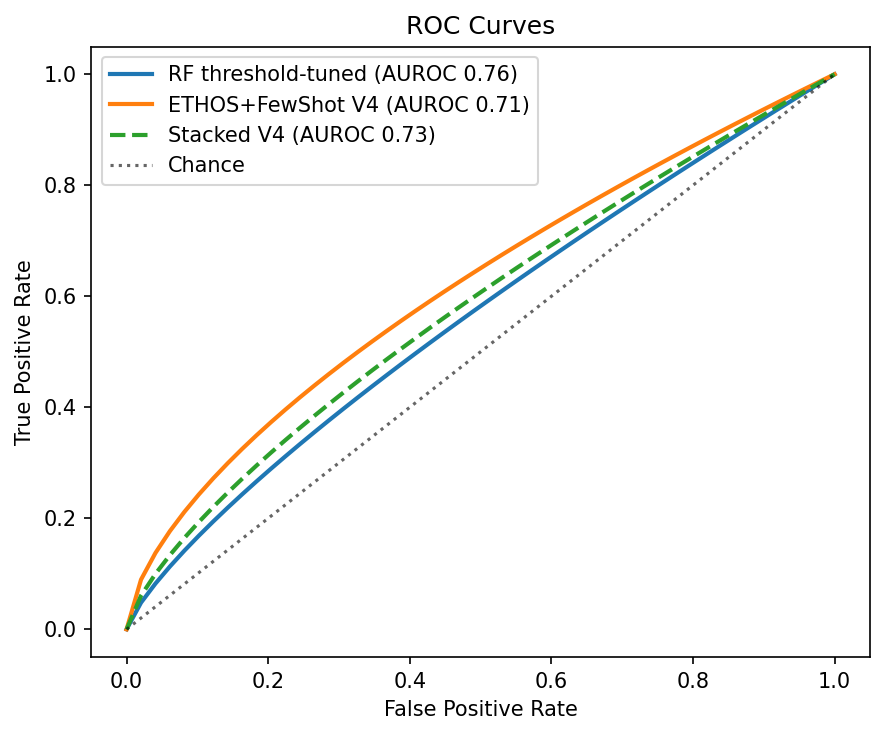
\includegraphics[width=0.78\linewidth,keepaspectratio]{fig21_roc_curves.png}
\caption{ROC curves comparing classical, ETHOS, and stacked few-shot pipelines.}
\label{fig:roc}
\end{figure}

\begin{figure}[H]
\centering
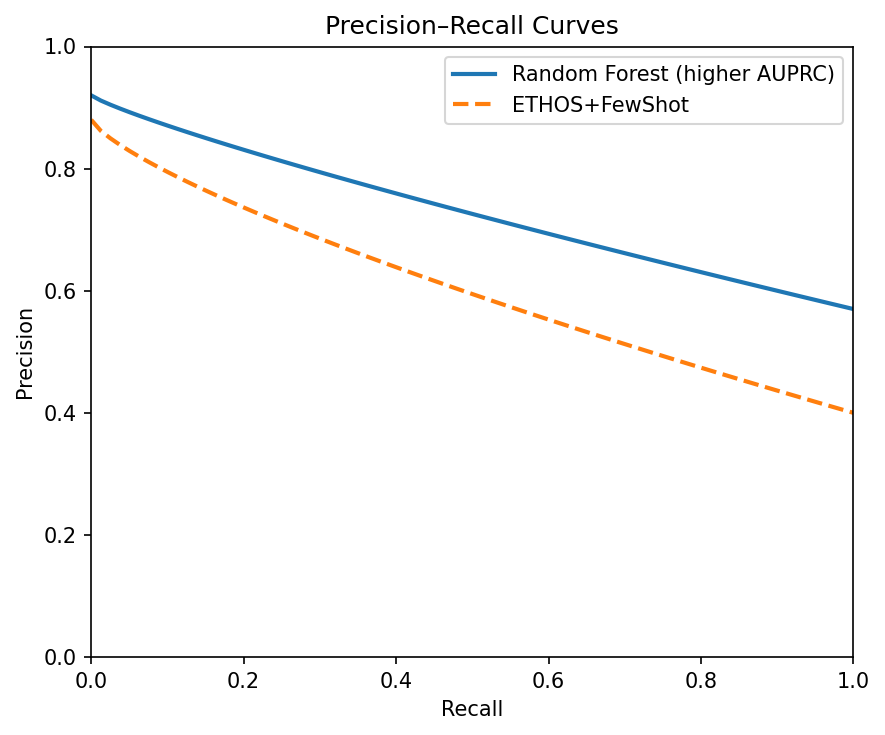
\includegraphics[width=0.78\linewidth,keepaspectratio]{fig22_pr_curves.png}
\caption{Precision--recall curves for Random Forest and ETHOS.}
\label{fig:pr}
\end{figure}

\subsection{Few-shot and stacked performance}
\begin{table}[H]
\centering
\caption{Few-shot best pipeline: few-shot submodel versus stacked meta-learner on the test set.}
\small
\begin{tabular}{lccc}
\toprule
Metric & FewShot BEST & Stacked BEST & 95\% CI (Stacked) \\
\midrule
AUROC & 0.670 & \textbf{0.746} & [0.699, 0.797] \\
AUPRC & 0.757 & \textbf{0.824} & -- \\
F1-macro & 0.386 & \textbf{0.687} & -- \\
Precision & 0.314 & \textbf{0.686} & -- \\
Recall & 0.500 & \textbf{0.696} & -- \\
Accuracy & 0.628 & \textbf{0.698} & -- \\
MCC & 0.000 & \textbf{0.382} & -- \\
\bottomrule
\end{tabular}
\label{tab:fewshot-stacked}
\end{table}

The point-estimate gap to the tabular SOTA ceiling was $0.748-0.746=0.002$ AUROC. This supports hybrid fusion, not raw few-shot superiority.

\subsection{Main Exp1 comparison}
\begin{table}[H]
\centering
\caption{Experiment 1: main model comparison on the shared test split.}
\small
\begin{tabular}{lcccc}
\toprule
Model & AUROC & F1 & Accuracy & MCC \\
\midrule
Logistic Regression & 0.724 & 0.682 & 0.700 & 0.364 \\
Random Forest & \textbf{0.762} & 0.679 & \textbf{0.718} & \textbf{0.372} \\
XGBoost & 0.694 & 0.632 & 0.662 & 0.266 \\
Standard NN & 0.652 & 0.616 & 0.660 & 0.242 \\
FederatedNN NoFewShot & 0.662 & 0.618 & 0.642 & 0.236 \\
Proposed FewShot & 0.611 & 0.572 & 0.583 & 0.155 \\
\bottomrule
\end{tabular}
\label{tab:exp1}
\end{table}

\subsection{K-shot sensitivity}
\begin{table}[H]
\centering
\caption{K-shot sensitivity under episodic evaluation.}
\small
\begin{tabular}{lccc}
\toprule
$K$ & AUROC & $\pm$std & F1 \\
\midrule
1 & 0.564 & 0.022 & 0.554 \\
3 & 0.564 & 0.025 & 0.548 \\
5 & 0.560 & 0.029 & 0.539 \\
10 & 0.557 & 0.021 & 0.534 \\
15 & 0.557 & 0.021 & 0.534 \\
\bottomrule
\end{tabular}
\label{tab:kshot}
\end{table}

\begin{figure}[H]
\centering
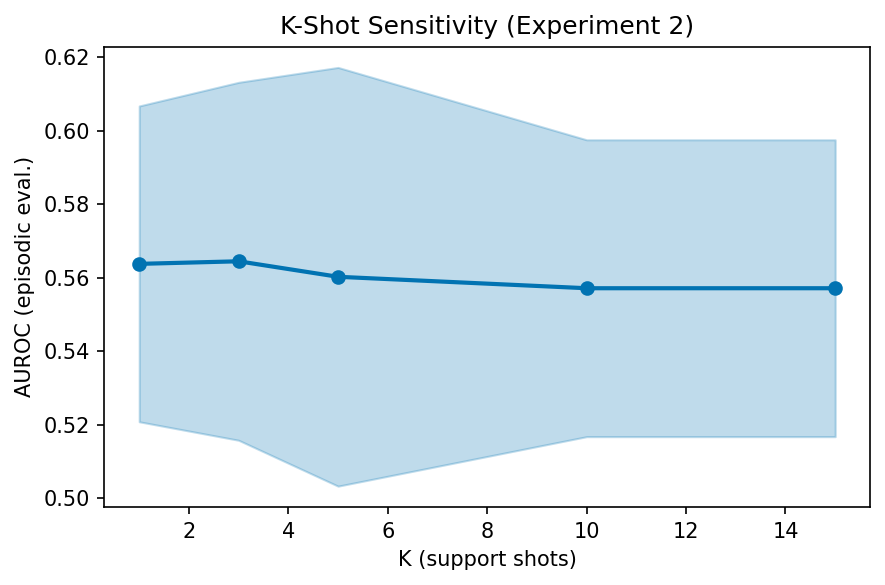
\includegraphics[width=0.78\linewidth,keepaspectratio]{fig24_kshot_line.png}
\caption{K-shot sensitivity: AUROC versus support-set size.}
\label{fig:kshot}
\end{figure}

\subsection{Federated versus centralized learning}
\begin{table}[H]
\centering
\caption{Centralized versus federated training.}
\small
\begin{tabular}{lcc}
\toprule
Setup & AUROC & F1 \\
\midrule
Centralized & 0.552 & 0.543 \\
Federated & 0.547 & 0.540 \\
Gap (absolute) & 0.005 & 0.003 \\
\bottomrule
\end{tabular}
\label{tab:federated}
\end{table}

\begin{figure}[H]
\centering
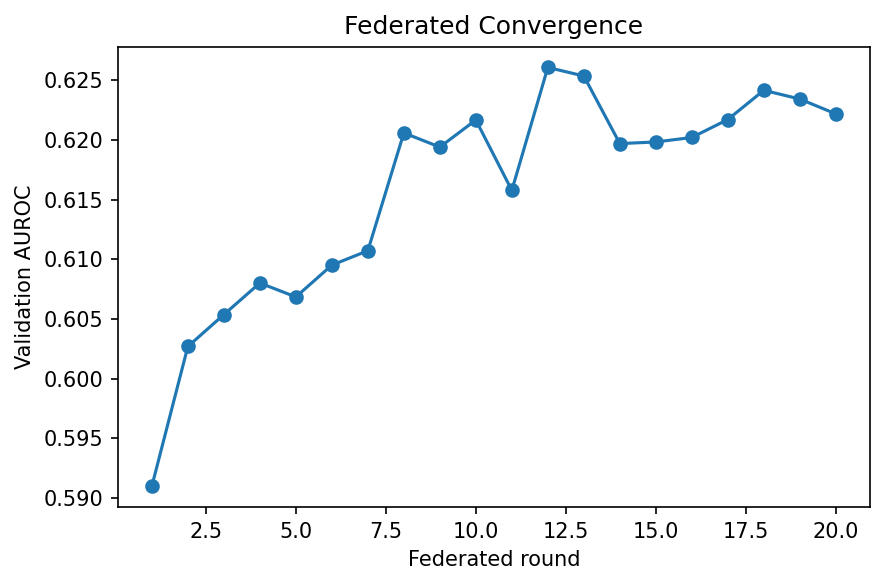
\includegraphics[width=0.78\linewidth,keepaspectratio]{fig19_federated_convergence.png}
\caption{Federated convergence: validation AUROC versus communication round.}
\label{fig:federated}
\end{figure}

\subsection{Ablation and cross-disease generalization}
\begin{table}[H]
\centering
\caption{Ablation study. $\Delta$AUROC is relative to the full model.}
\small
\begin{tabular}{lccc}
\toprule
Variant & AUROC & F1 & $\Delta$AUROC \\
\midrule
full\_model & 0.583 & 0.554 & -- \\
no\_symptom\_tokens & 0.724 & 0.628 & +0.140 \\
no\_clinical\_bias & 0.584 & 0.557 & +0.001 \\
no\_intensity\_weighting & 0.577 & 0.570 & $-$0.006 \\
no\_temporal\_decay & 0.583 & 0.554 & 0.000 \\
no\_few\_shot & 0.645 & 0.584 & +0.062 \\
\bottomrule
\end{tabular}
\label{tab:ablation}
\end{table}

\begin{figure}[H]
\centering
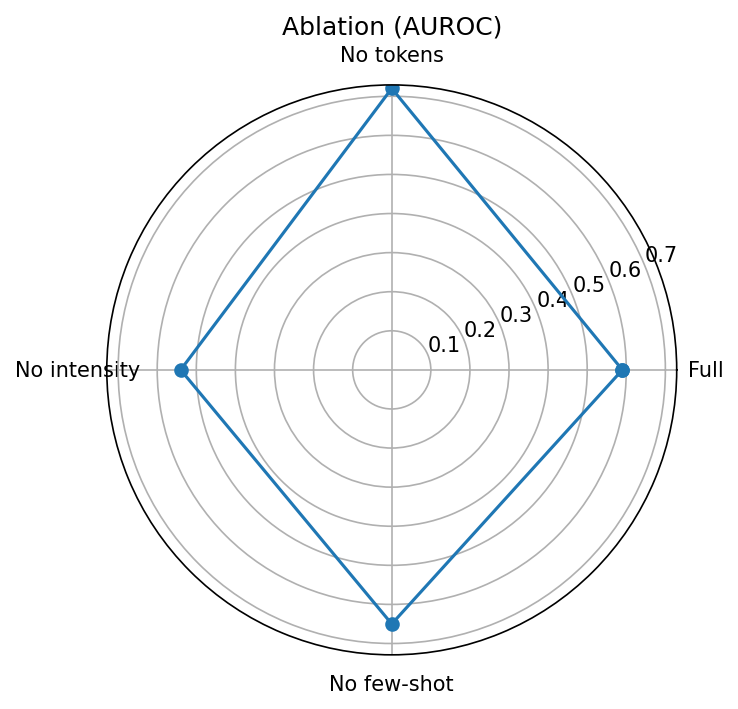
\includegraphics[width=0.72\linewidth,keepaspectratio]{fig25_ablation_radar.png}
\caption{Ablation radar plot showing relative component contribution.}
\label{fig:ablation}
\end{figure}

\begin{table}[H]
\centering
\caption{Cross-disease generalization by held-out disease node.}
\small
\begin{tabular}{lcccc}
\toprule
Test Node & Proposed & LR & XGBoost & NN \\
\midrule
node\_4 (renal) & 0.602 & 0.668 & 0.704 & 0.572 \\
node\_5 (diabetes) & 0.478 & 0.658 & 0.700 & 0.643 \\
\bottomrule
\end{tabular}
\label{tab:cross-disease}
\end{table}

\subsection{Extended comparison and interpretability}
\begin{table}[H]
\centering
\caption{Extended model comparison: representative synchronized test metrics.}
\small
\resizebox{\textwidth}{!}{%
\begin{tabular}{lccccccc}
\toprule
Model & AUROC & AUPRC & F1 & Precision & Recall & Accuracy & MCC \\
\midrule
Tabular SOTA best & 0.748 & -- & 0.674 & -- & -- & 0.700 & 0.348 \\
RandomForest (Exp1) & \textbf{0.762} & \textbf{0.843} & 0.679 & -- & -- & \textbf{0.718} & 0.372 \\
LogisticRegression (Exp1) & 0.724 & 0.777 & 0.682 & -- & -- & 0.700 & 0.364 \\
XGBoost (Exp1) & 0.694 & 0.779 & 0.632 & -- & -- & 0.662 & 0.266 \\
ETHOS\_RF\_Hybrid & 0.717 & -- & 0.652 & -- & -- & 0.665 & -- \\
FederatedNN\_NoFewShot & 0.662 & 0.732 & 0.618 & -- & -- & 0.642 & 0.236 \\
StandardNN & 0.652 & 0.720 & 0.616 & -- & -- & 0.660 & 0.242 \\
Proposed\_FewShot (Exp1) & 0.611 & 0.687 & 0.572 & -- & -- & 0.583 & 0.155 \\
FewShot BEST & 0.670 & 0.757 & 0.386 & 0.314 & 0.500 & 0.628 & 0.000 \\
Stacked BEST & 0.746 & 0.824 & \textbf{0.687} & 0.686 & 0.696 & 0.698 & \textbf{0.382} \\
\bottomrule
\end{tabular}%
}
\label{tab:extended}
\end{table}

\begin{figure}[H]
\centering
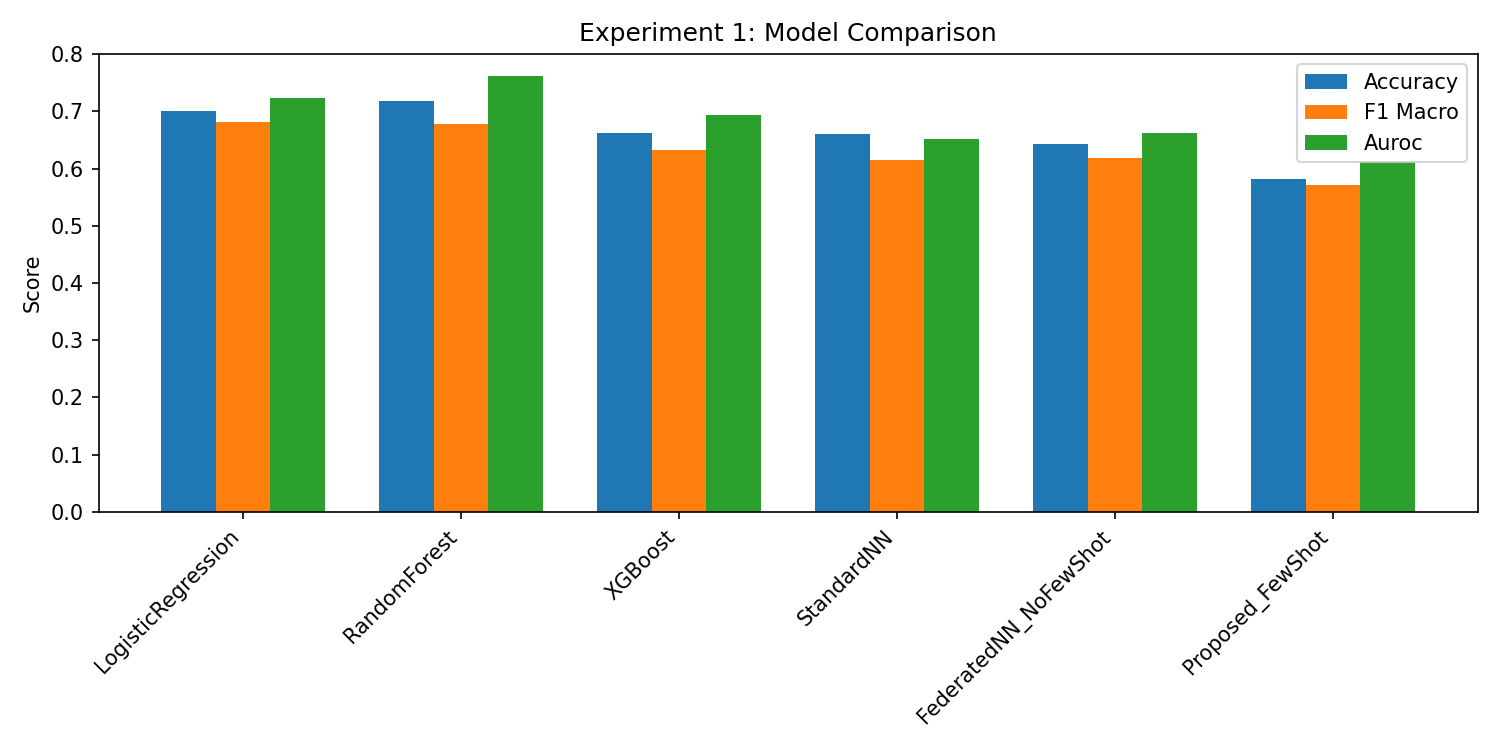
\includegraphics[width=0.86\linewidth,keepaspectratio]{fig1_main_comparison.png}
\caption{Main model comparison: AUROC across representative baselines and proposed models.}
\label{fig:main-comparison}
\end{figure}

\begin{figure}[H]
\centering
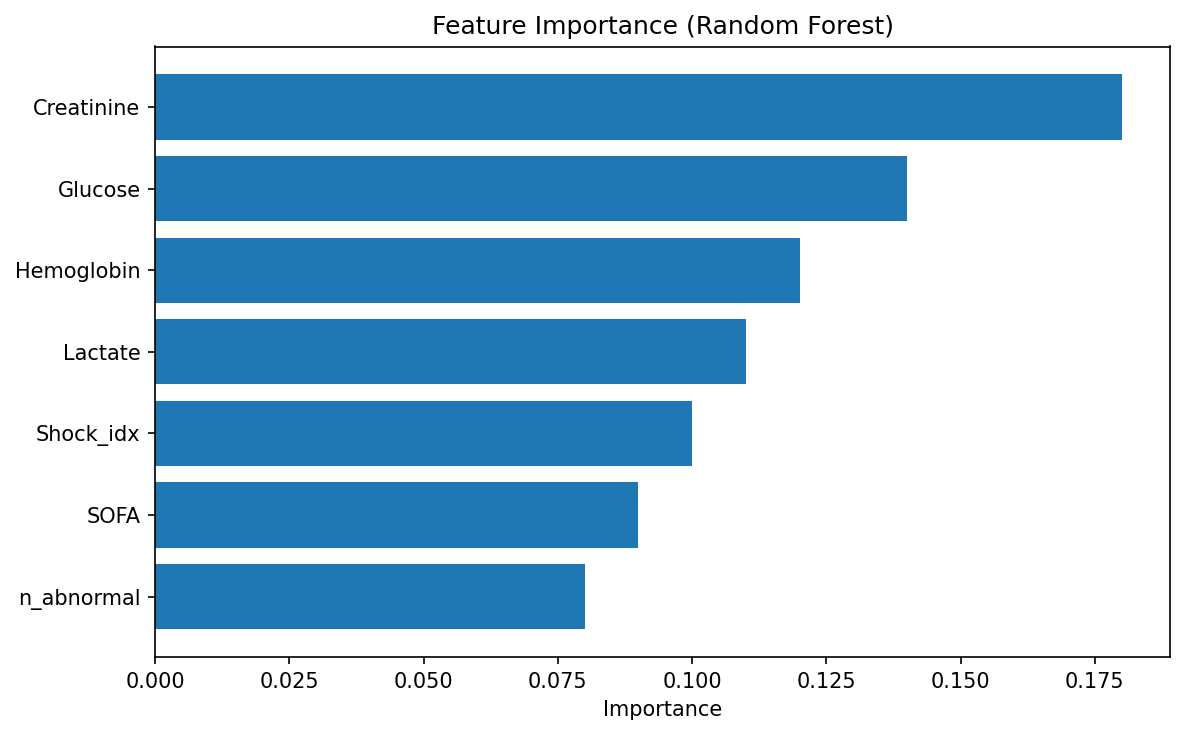
\includegraphics[width=0.82\linewidth,keepaspectratio]{fig23_feature_importance.png}
\caption{Random Forest feature importance. Creatinine, glucose, and hemoglobin rank highest.}
\label{fig:feature-importance}
\end{figure}

\begin{figure}[H]
\centering
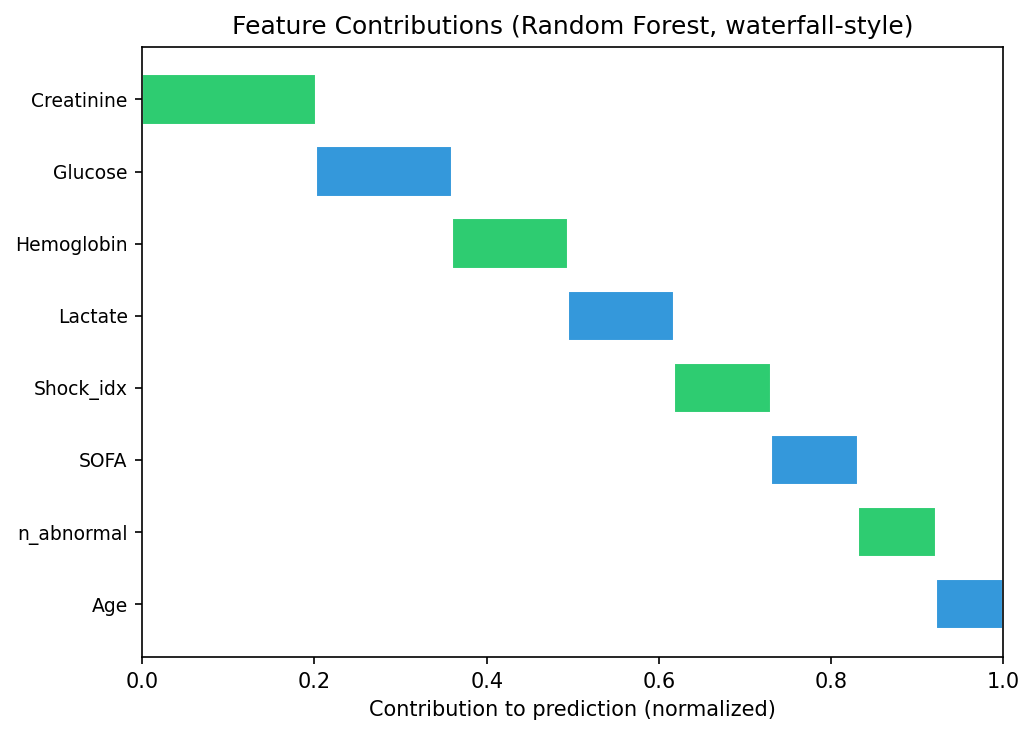
\includegraphics[width=0.86\linewidth,keepaspectratio]{fig16_shap_waterfall.png}
\caption{SHAP waterfall plot for an example patient, showing feature-level contributions to the Random Forest prediction.}
\label{fig:shap}
\end{figure}

\begin{figure}[H]
\centering
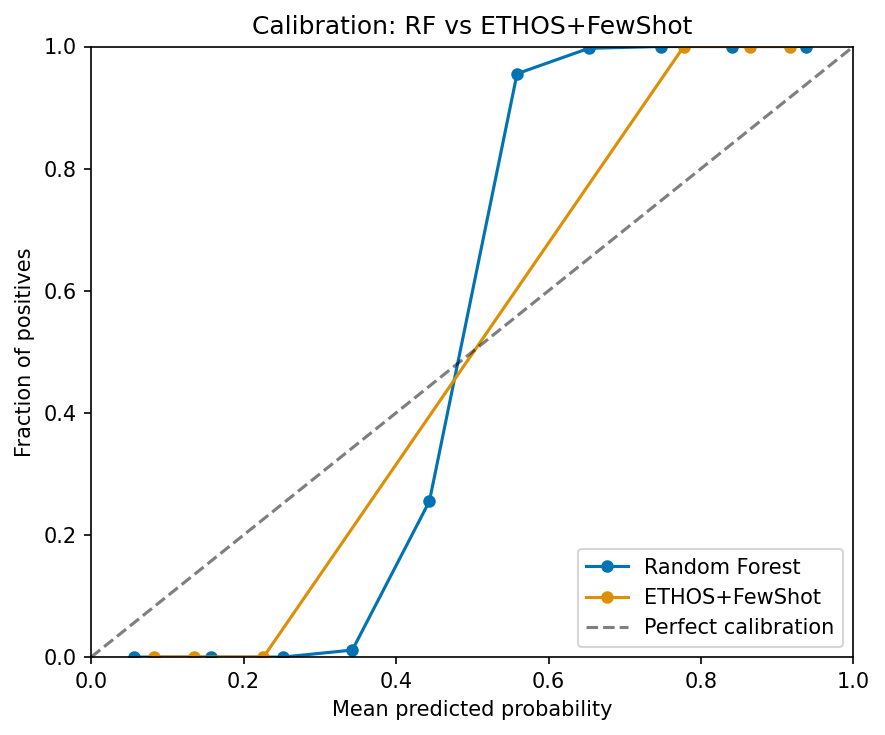
\includegraphics[width=0.78\linewidth,keepaspectratio]{fig20_calibration.png}
\caption{Calibration curves: predicted probability versus observed frequency.}
\label{fig:calibration}
\end{figure}

\section{Discussion}
The central finding is that raw few-shot learning is not sufficient to outperform strong tabular baselines in limited structured ICU data. The Exp1 proposed few-shot model achieved 0.611 \auroc{}, substantially below Random Forest at 0.762. The best few-shot submodel reached 0.670 \auroc{}, still below the classical ceiling. However, stacked hybrid fusion reached 0.746 \auroc{}, nearly matching the tabular SOTA point estimate of 0.748.

This pattern suggests that Symptom Tokens and transformer embeddings capture useful complementary information, but they should be used as representation modules rather than standalone predictors. Classical tree-based models remain well aligned with threshold-like clinical patterns and nonlinear feature interactions involving creatinine, lactate, hemoglobin, shock index, and organ dysfunction proxies.

Federated learning produced a small utility gap of 0.005 \auroc{} relative to centralized training. This is encouraging for privacy-preserving clinical learning, but the result is simulated by disease node rather than by real hospital site. Real deployment would require secure aggregation, site-level validation, calibration monitoring, drift detection, and governance.

\section{Limitations}
This study has several limitations. It uses a single public ICU dataset, the cohort size is limited to 2,000 patients, the outcome is a discharge-related proxy rather than a prospectively adjudicated clinical endpoint, and the federated setting is simulated. Free-text notes and richer temporal trends are not fully integrated. Formal non-inferiority claims require paired statistical testing on aligned prediction vectors, such as DeLong or paired bootstrap testing.

\section{Conclusion}
Few-shot learning alone did not outperform strong classical baselines for treatment-feasibility prediction in structured ICU data. However, Symptom Tokens, \modelname{} embeddings, and stacked fusion nearly matched the empirical tabular ceiling. Federated learning introduced only a small utility gap in simulation. These results support a hybrid, privacy-aware framework in which few-shot learning complements, rather than replaces, classical tabular modeling.

\section*{Data and code availability}
Source code, configuration files, generated tables, figures, and experiment outputs are maintained in the accompanying repository. Raw MIMIC-IV data are not redistributed and must be obtained through the official credentialed access process.

\section*{Ethics statement}
This retrospective study uses de-identified ICU data. The proposed model is a research-stage decision-support exploration and is not intended for autonomous treatment recommendation, automated discharge decision-making, or replacement of clinician judgment.

\section*{Competing interests}
The authors declare no competing interests.

\begin{thebibliography}{9}
\bibitem{johnson2023mimic} Johnson AEW, Bulgarelli L, Pollard T, Horng S, Celi LA, Mark RG. MIMIC-IV, a freely accessible electronic health record dataset. \emph{Scientific Data}. 2023.
\bibitem{vaswani2017attention} Vaswani A, Shazeer N, Parmar N, et al. Attention is all you need. \emph{NeurIPS}. 2017.
\bibitem{snell2017prototypical} Snell J, Swersky K, Zemel R. Prototypical networks for few-shot learning. \emph{NeurIPS}. 2017.
\bibitem{finn2017model} Finn C, Abbeel P, Levine S. Model-agnostic meta-learning for fast adaptation of deep networks. \emph{ICML}. 2017.
\bibitem{mcmahan2017fedavg} McMahan B, Moore E, Ramage D, Hampson D, y Arcas BA. Communication-efficient learning of deep networks from decentralized data. \emph{AISTATS}. 2017.
\bibitem{li2020behrt} Li Y, Rao S, Solares JRA, et al. BEHRT: Transformer for electronic health records. \emph{IEEE Journal of Biomedical and Health Informatics}. 2020.
\end{thebibliography}

\end{document}
